\documentclass[review]{elsarticle}

\usepackage{lineno,hyperref}
\modulolinenumbers[5]

\journal{Eugène Syriani, University of Montreal}

%%%%%%%%%%%%%%%%%%%%%%%
%% Elsevier bibliography styles
%%%%%%%%%%%%%%%%%%%%%%%
%% To change the style, put a % in front of the second line of the current style and
%% remove the % from the second line of the style you would like to use.
%%%%%%%%%%%%%%%%%%%%%%%

%% Numbered
%\bibliographystyle{model1-num-names}

%% Numbered without titles
%\bibliographystyle{model1a-num-names}

%% Harvard
%\bibliographystyle{model2-names.bst}\biboptions{authoryear}

%% Vancouver numbered
%\usepackage{numcompress}\bibliographystyle{model3-num-names}

%% Vancouver name/year
%\usepackage{numcompress}\bibliographystyle{model4-names}\biboptions{authoryear}

%% APA style
%\bibliographystyle{model5-names}\biboptions{authoryear}

%% AMA style
%\usepackage{numcompress}\bibliographystyle{model6-num-names}

%% `Elsevier LaTeX' style
\bibliographystyle{elsarticle-num}
%%%%%%%%%%%%%%%%%%%%%%%

\begin{document}

\begin{frontmatter}

\title{Visual Parametric Maze Generator DSL \tnoteref{mytitlenote}}
\tnotetext[mytitlenote]{Full source code is available on \href{https://github.com/Thealoe/ParametrizedMazeGen}{GitHub}.}

%% Group authors per affiliation:
\author{Corentin Moiny\fnref{myfootnote}}
\address{304, 5e Avenue Mailloux, La Pocatière. Quebec. Canada}
\fntext[myfootnote]{2020}

%% or include affiliations in footnotes:
\author[mymainaddress]{University of Montreal}
\ead{corentin.moiny@umontreal.ca}

\address[mymainaddress]{2900 Edouard Montpetit Blvd, Montreal, Quebec. Canada}

\begin{abstract}
(TODO) - This is a test abstract again and again.
\end{abstract}

\begin{keyword}
MDE \sep Maze \sep Generator \sep Parametric \sep Python \sep Epsilon \sep DSL \sep Java \sep Visual
\MSC[2010] 00-01\sep  99-00
\end{keyword}

\end{frontmatter}

\linenumbers

\section{Introduction}

\paragraph{A}
In the context of our Model-driven Engineering project assignment, I was charged to design a visual DSL to generate parametric mazes using a external Python program that I have also implemented. The goal of this project is to empower parameters understanding with the DSL and than produce probabilistic mazes. With this approach, anyone could generate maze with minimal or no engineering knowledge. Parametric maze generation is not a new concept, our approach was highly inspired by Design-Centric Maze Generation by Paul Hyunjin Kim and al\cite{kim_design-centric_2019}. From this paper we used the maze cells concept where each one of them represent a 3x3 tiles on the maze. We also used the same of types of rates (and more) as in the paper and used them with a probabilist approach. 

\paragraph{B}
(TODO) - Details of the sections presented

\section{Solution}

In this section, I give details on the solution choices used and the purposes behind theses.

\subsection{DSL}

The domain specific language represent the parameters used to generate the maze. Presented as a visual syntax in Figure \ref{fig:model}, it contains four types of generator. From left to right, generators are represented as blue rectangles: (1) \textit{RGen} is the first step of the maze generation, it gives the initial borders of the maze using a row count (\textit{RC}) and a column count (\textit{CC}) represented as red squares. (2) \textit{FPGen} inject maze cells in this initial shape to force pattern, it allows users to create drawing in the maze. It is represented as orangish square (\textit{Marked 15 with a CP}) where a point is defined inside of it. In this case we only force a single cell. (3) ... (TODO)

\begin{figure}
	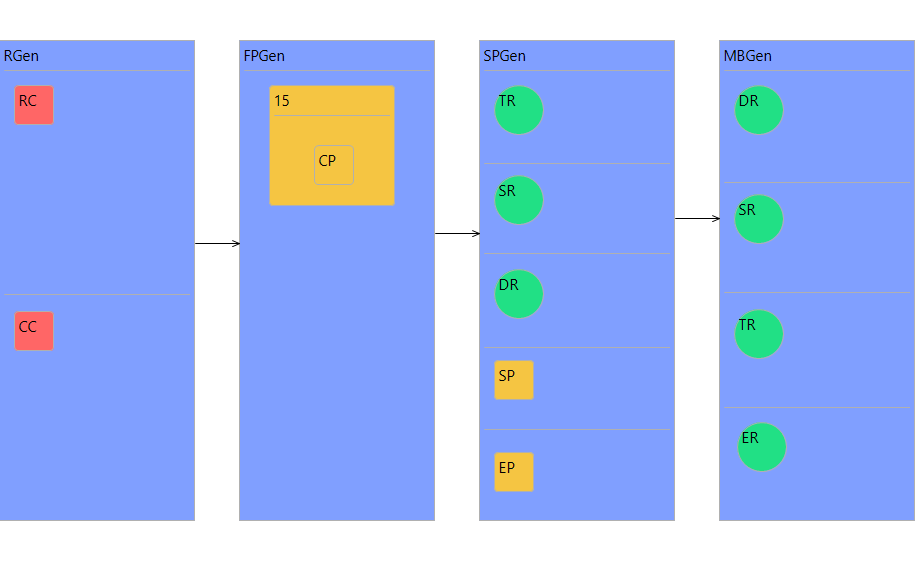
\includegraphics[width=\linewidth]{model.png}
	\caption{A model instance from the DSL}
	\label{fig:model}
\end{figure}

\subsection{Generator}

\section{Evaluation}

\section{Related Work}

\section{Conclusion}

\bibliography{mybibfile}

\end{document}